\section*{Front-End Web Development with React}

This course provide an introduction to the React framework, its components and some basic elements like routing, forms and animations. Shared state management, with the corresponding tools like Redux, is another important topic covered alongside fetching data.

\subsection*{Single Page Application}
A traditional website is a collection of pages and resources that are fetched to the server for each page that is navigated. Even if a lot of pages have part i common, like footer or header, they are requested entirely every time a new page is navigated. In a Single Page Application (SPA) the entire website is downloaded at first, then only the data that changes are re-downloaded from the server. A SPA enable to deliver a user experience closer to a desktop application, does not need to be entirely reloaded and allows the browser to re-render only the parts that are changed. 
Some downside of a SPA is that Search Engine Optmiziation (SEO) is more difficult to achieve and the initial page load can be slower than a traditional website.


\subsection*{React Overview}

React is a JavaScript library for building component-based user interfaces using a declarative approach. React focuses only on user interface and is designed for speed, simplicity and scalability.

A React component is a JavaScript class or function that  is imported from the React Module. It is then rendered using the React's rendering function \texttt{ReactCOM.render(...)}.

\subsubsection*{Components}
A component is an indipendent and reusable set of React elements that should appear on screen. Every component can accepts any input and is composed of React tags, that always start with a capital letter, and native tags, which start with lowercase letters and are treated as DOM tags.
Every component has a local state which can hold multiple information that can be passed to children components using \texttt{props}. The state is an immutable object that can be updated using the \texttt{setState(...)} directive. This function accept the property to update and merge it with the actual state. Only class components can have a local state. The state must never be manipulated directly.

Handling event is possible in a similar way as on DOM elements:

\begin{figure}[h]
    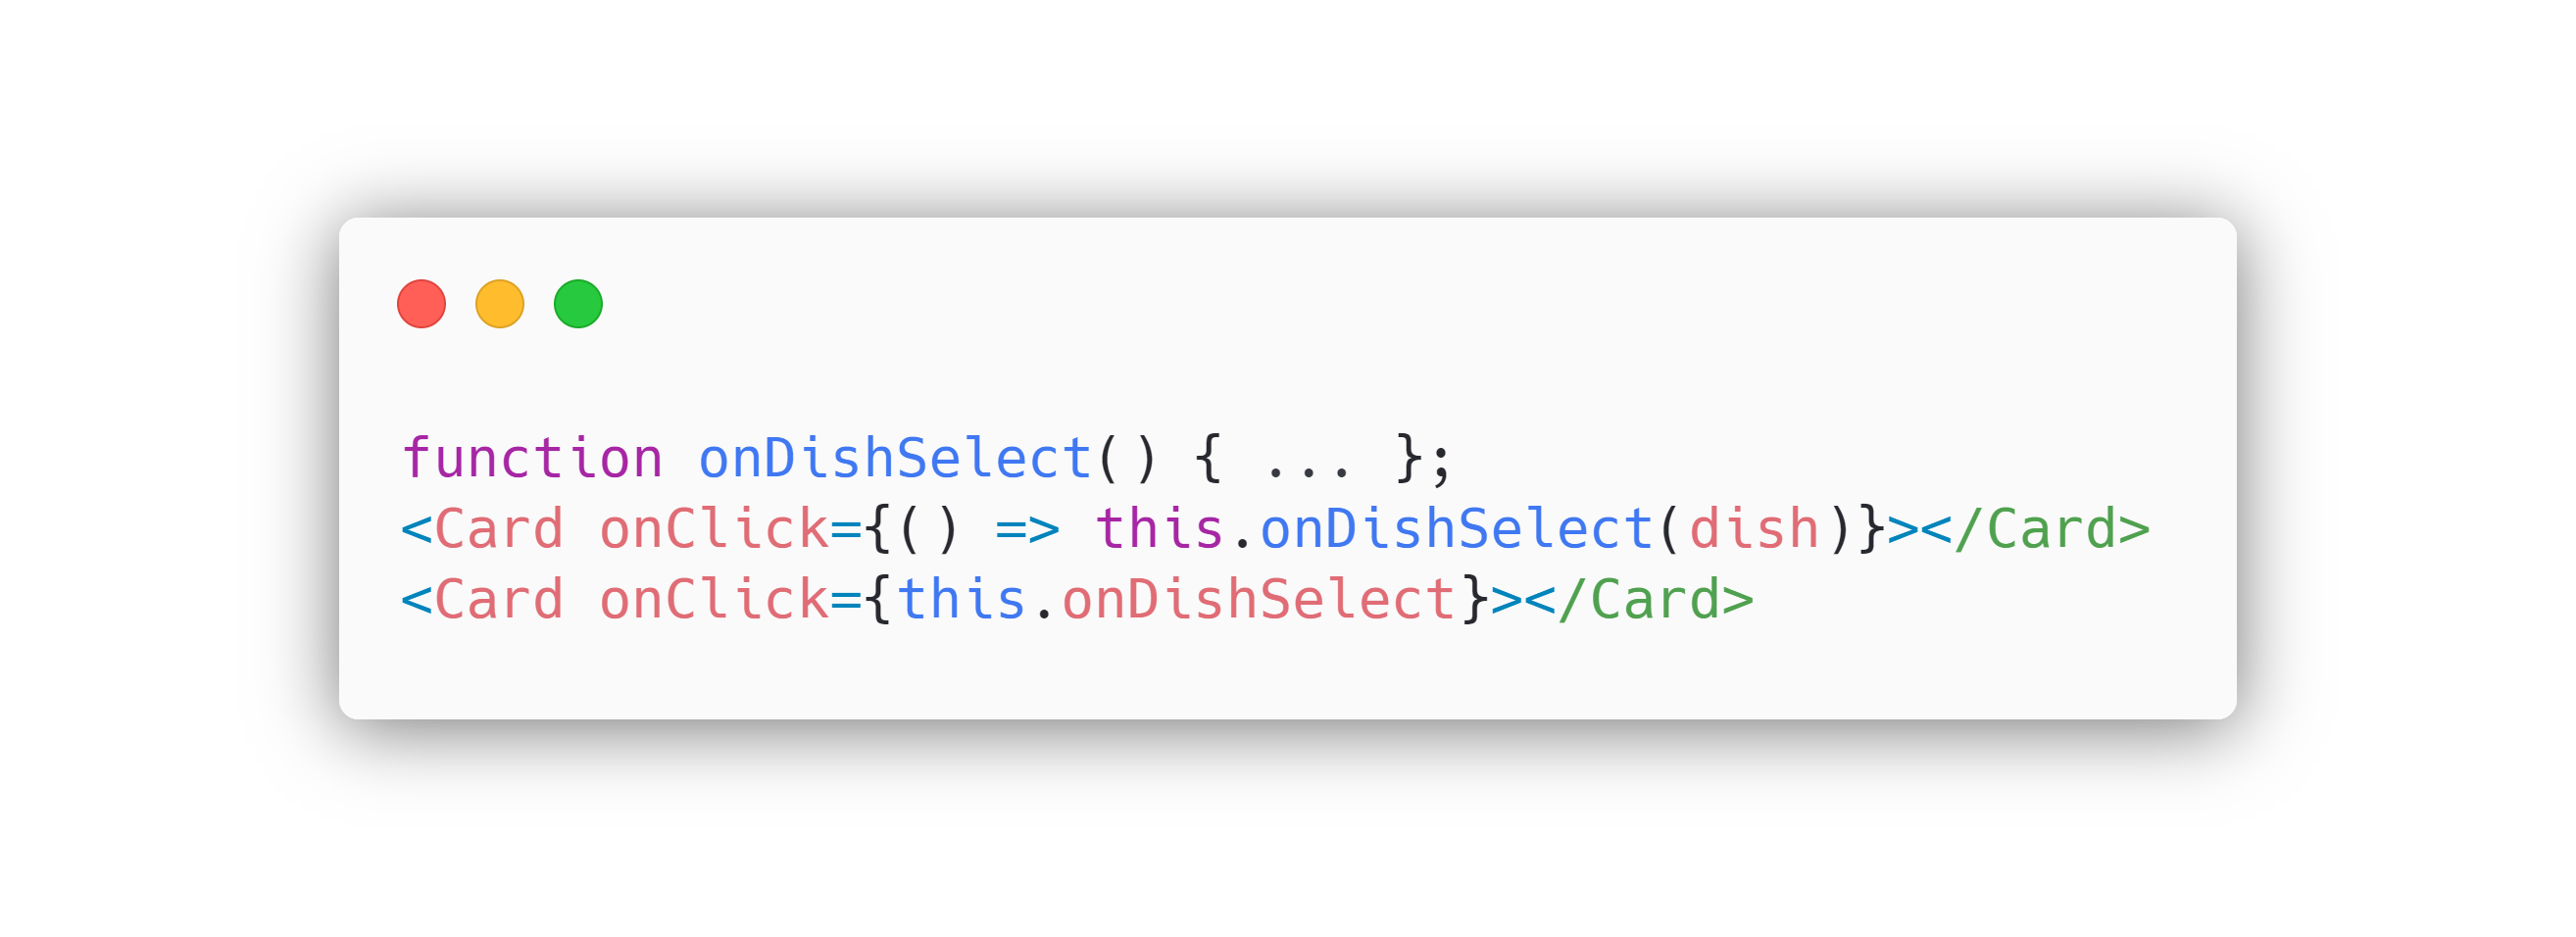
\includegraphics[width=\textwidth]{assets/react-event-handling.png}
    \caption{Event handling when clicking on div}
    \label{fig:event-handling}
\end{figure}

In Figure \ref{fig:event-handling} is possible to see how map a function to a click event on the React element \texttt{Card}.

\subsubsection*{Lifecycle}
React provides life cycle hooks/methods that can be invoked to perform certain operations. Component is created and then mounted in the application and when it's not required anymore is unmounted. There are three stages of lifecycle: mounting, updating and unmounting. Each stage provide, when component is declared as class, several methods like a construcor (mounting), \texttt{componentDidMount()} (called after mounting is finished), \texttt{render()} (call when rendering UI) and many others.

\subsubsection*{Functonal vs Class}
Until the release of \texttt{React 16.8} in 2018 there were two ways of declaring a component: class component or functional component. Functional components are s JavaScript function that returns a React element, can receive props but cannot provide local state or lifecycle hooks. 
\begin{figure}
    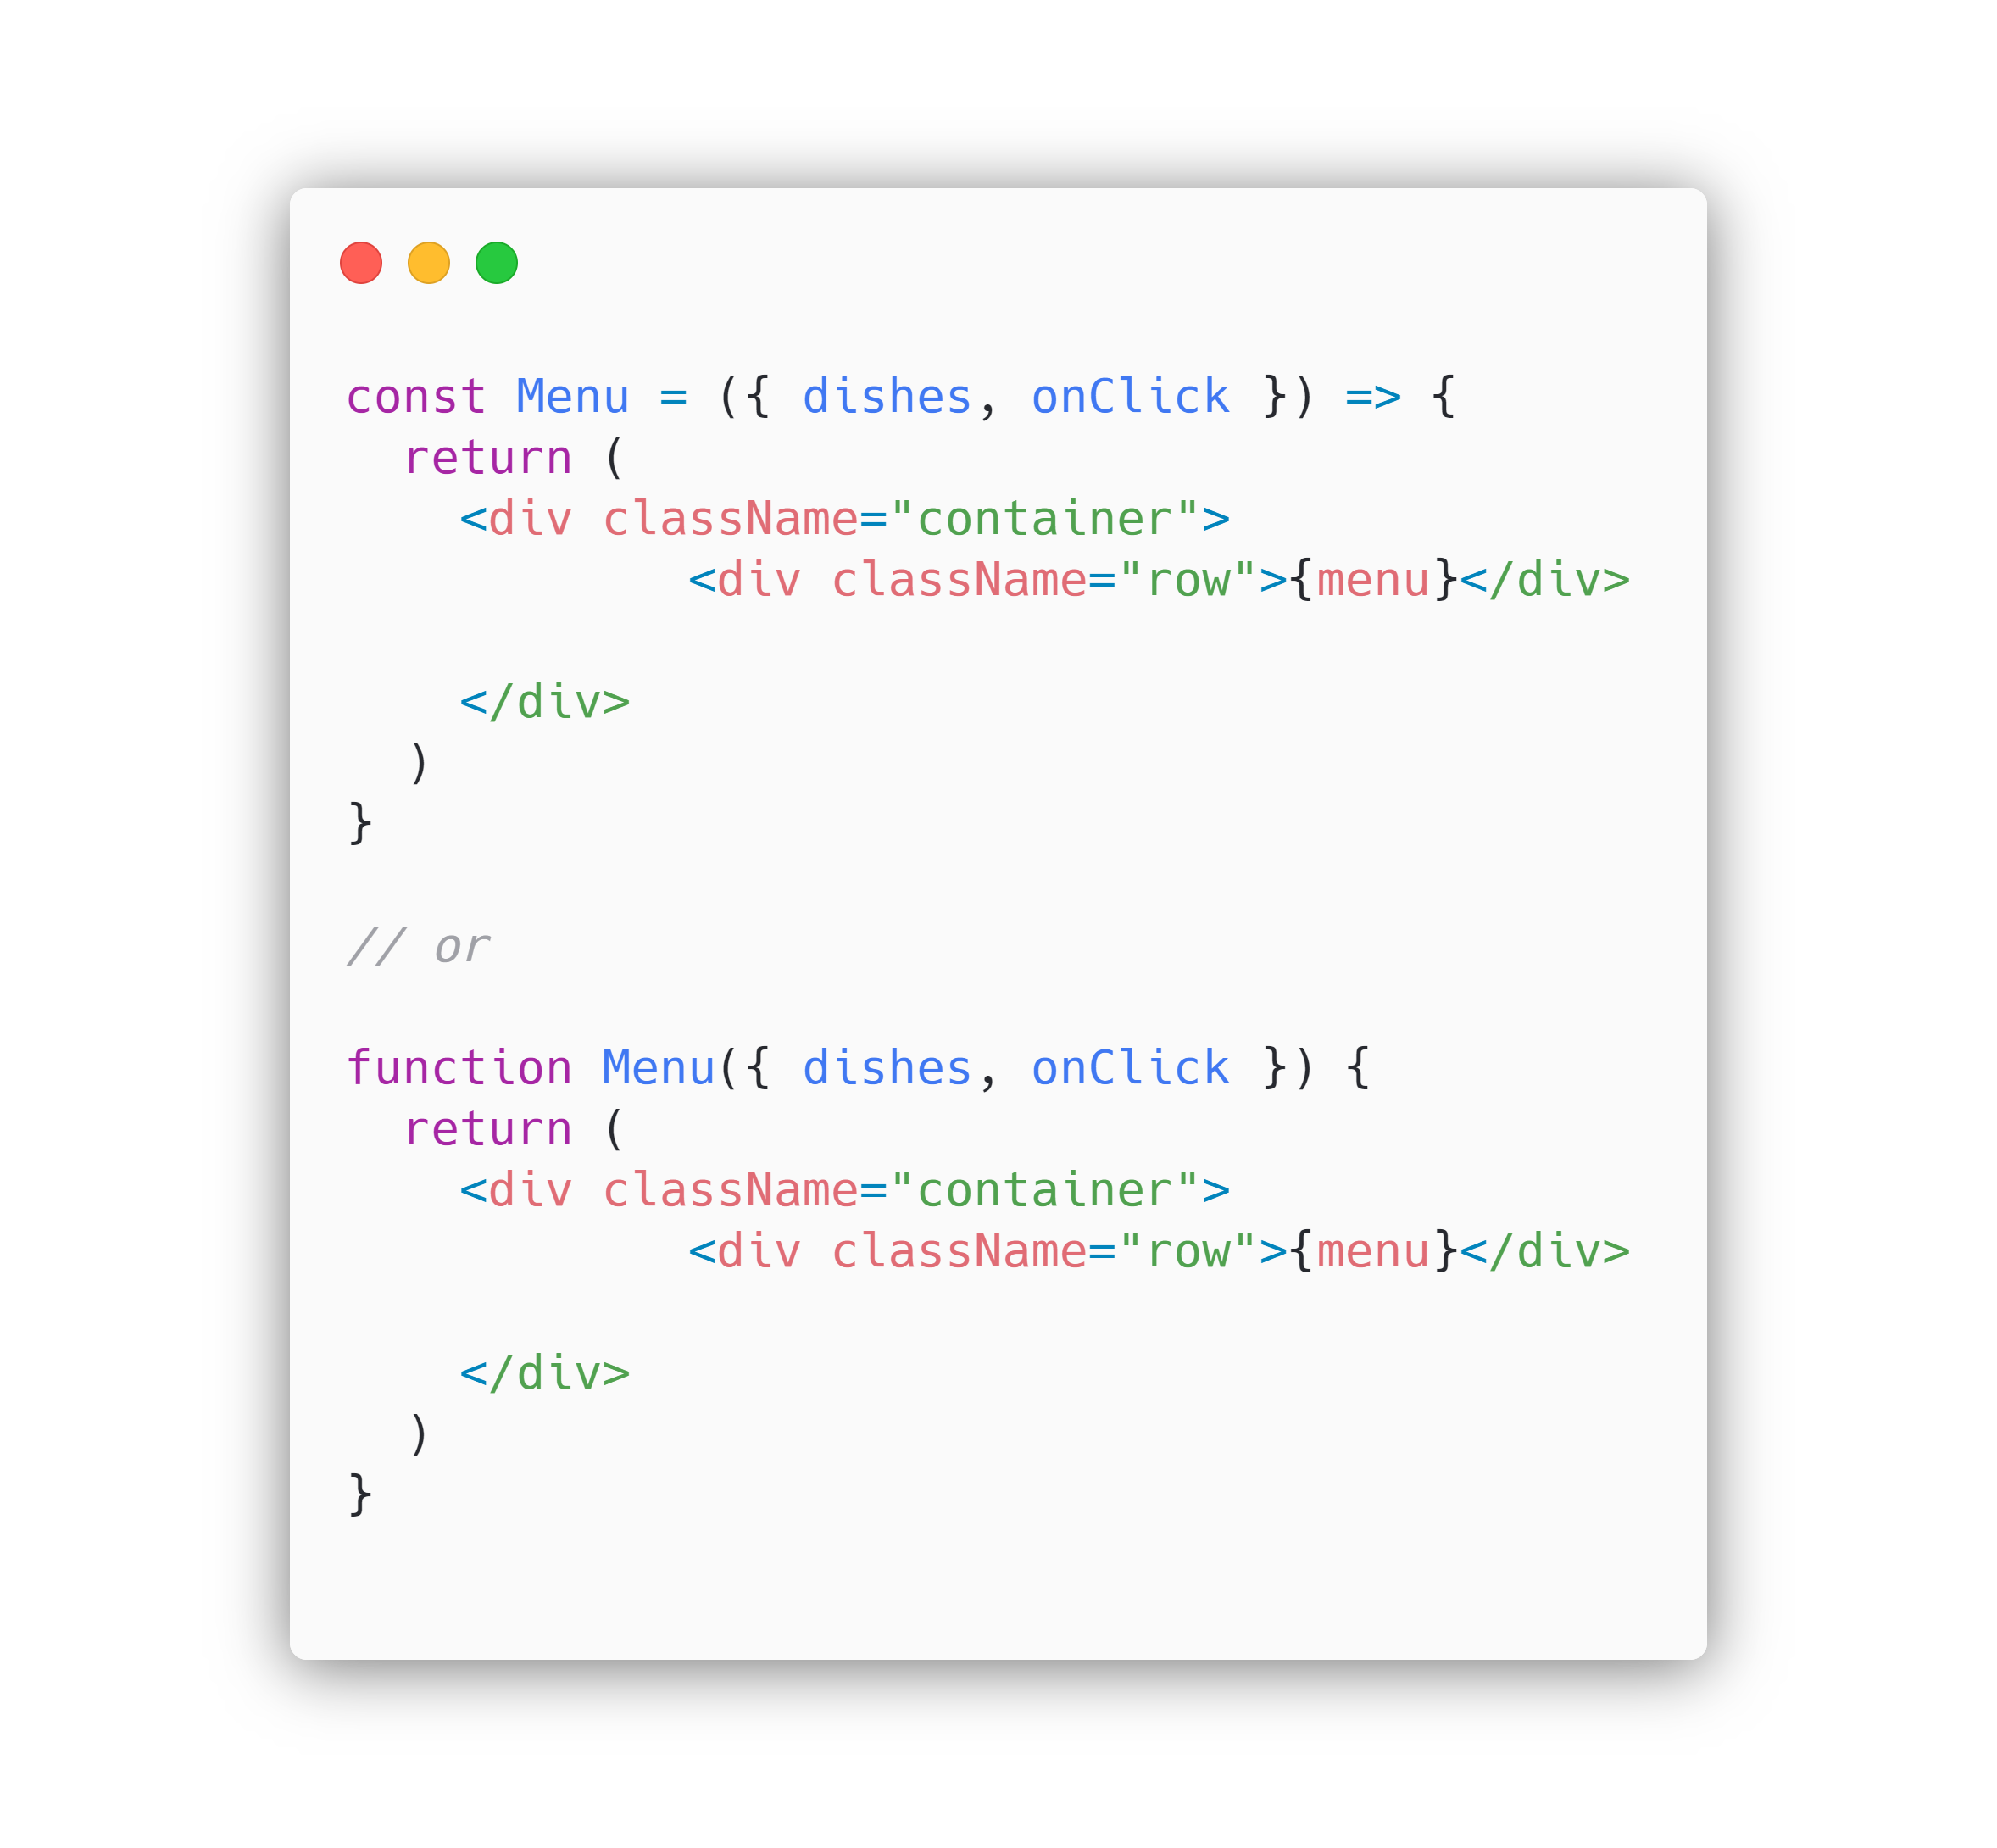
\includegraphics[width=\textwidth]{assets/class-vs-functional.png}
    \caption{Ways to define a functional components as function or arrow function}
\end{figure}

In React 16.8 it was introduced React Hooks to use lifecycle hooks also in functional component. This topic is not covered in courses, but will be discussed in the appendix of this document.

\subsubsection*{Document Object Model}
In the browser there is an object called \texttt{Browser DOM} (Document Object Model) and is the representation of the structure and data of a webpage. React uses a lightweight version of DOM called \texttt{Virtual DOM}, which uses an in-memory tree data structure of plain JavaScript objects, is extremely fast to manipulate compared to browser DOM and is fully recreated on every setState. 

There is a diffing algorithm that detect which nodes are changed and updates the only the minimum number of components in the sub-tree that is updated.

\subsubsection*{React Router}
React Router gives the ability to navigate between views using links. It's a module that need to be additionally installed into the React application called \texttt{react-router-dom}. It is a collection of navigational components that enable navigation among views and support a browser-based bookmarkable URLs to navigate in the web app. It is also possible to pass optional parameters.
This dependency allows you to use the \textit{<BrowserRouter>} tag, which enables navigation between multiple pages.
There is also the possibility to use \textit{<Route>} to specify the path to a page or component, or \textit{<Switch>} to group several routers and route the page according to state (like any switch).
Navigation is possible using \textit{<Link>} or \textit{<NavLink>}.

\subsubsection*{Parameters}
It is possible to pass parameters through the URL and pass it to the view, for example \textit{/menu/42} can be rendered in the view mapped to \textit{/menu} with an input parameter \textit{42}.

\subsubsection*{Forms}
In React there are two types of forms: controlled or unconttrolled.
Controlled forms are directly and bidirectionally tied to the state and every state mutation is associated with an handler.

An unconttrolled form is not tied to the state but holds the values internally in the DOM. It is possible to retrieve data, for example when sending information to a REST API, and does not need to have an handler for every state updte.


\subsection*{MVC Framework}
A Model-View-Controller is an architectural pattern commonly used to allow reusable components, isolate logic from user interface and permit indipendent development, testing and maintenance. 
The \textit{Model} part is normally used to manage behaviour and data, respond to requests about state or instruction to change state and notify the view when there is a change in the state.
The \textit{View} is used to present the information to the user in a user face.
A \textit{Controller} receive the input from the users, instructs the model on which action to perform and initiates a response.

React is not a full MVC framework (or its descendent Model-View View-Model), it only provides the presentation logic. The model and controller can be developed independently form the View using React.

\subsection*{Flux and Redux}
The Flux architecture is an alternative to the MVC approach. It is an unidirectional data flow, from an action to the view through a dispatcher and a store.
All updates have one unidirectional flow, the central unit is the store. If a view want to update the store it must use an action. It cannot update the store directly.
New action are propagated through the systems in response to user interaction and the dispatcher control all the changes that are made to the store.

\subsubsection*{Redux}
Redux is the place to store the state of the application and allow to have a consistent way to access it. Redux is widely adapted by the React community, but is not strictly connected to React itself. Redux make state mutations predictable.
The state is a single object and is the single source of truth, it is read only and the only way to change the state is through actions. Every change has to made with pure functions that takes the previous state and return a newly mutated one.
Using Redux is possible to implement logging utilities, api handling, undo/redo of a state and many other features.